\documentclass[a4paper,12pt]{article}
\usepackage[top = 2.5cm, bottom = 2.5cm, left = 2.5cm, right = 2.5cm]{geometry}
\usepackage[T1]{fontenc}
\usepackage[utf8]{inputenc}
\usepackage{multirow} 
\usepackage{booktabs} 
\usepackage{graphics}
\usepackage{graphicx}
\usepackage{subcaption}
\usepackage{mwe}
\usepackage[spanish]{babel}
\usepackage{setspace}
\setlength{\parindent}{0in}
\usepackage{float}
\usepackage{fancyhdr}
\usepackage{amsmath}
\usepackage{amssymb}
\usepackage{amsthm}
\usepackage{natbib}
\usepackage{graphicx}
\usepackage{subcaption}
\usepackage{booktabs}
\usepackage{etoolbox}
\usepackage{apalike}
\usepackage{minibox}
\usepackage{hyperref}
\usepackage{xcolor}
\usepackage{tcolorbox}
\usepackage{listings}
\usepackage{color}
\usepackage{verbatim}

\definecolor{mygreen}{rgb}{0,0.6,0}
\definecolor{mygray}{rgb}{0.5,0.5,0.5}
\definecolor{mymauve}{rgb}{0.58,0,0.82}

\lstset{ 
	backgroundcolor=\color{white},   % choose the background color; you must add \usepackage{color} or \usepackage{xcolor}; should come as last argument
	basicstyle=\footnotesize,        % the size of the fonts that are used for the code
	breakatwhitespace=false,         % sets if automatic breaks should only happen at whitespace
	breaklines=true,                 % sets automatic line breaking
	captionpos=b,                    % sets the caption-position to bottom
	commentstyle=\color{mygreen},    % comment style
	deletekeywords={...},            % if you want to delete keywords from the given language
	escapeinside={\%*}{*)},          % if you want to add LaTeX within your code
	extendedchars=true,              % lets you use non-ASCII characters; for 8-bits encodings only, does not work with UTF-8
	firstnumber=1000,                % start line enumeration with line 1000
	frame=single,	                   % adds a frame around the code
	keepspaces=true,                 % keeps spaces in text, useful for keeping indentation of code (possibly needs columns=flexible)
	keywordstyle=\color{blue},       % keyword style
	language=Octave,                 % the language of the code
	morekeywords={*,...},            % if you want to add more keywords to the set
	numbers=left,                    % where to put the line-numbers; possible values are (none, left, right)
	numbersep=5pt,                   % how far the line-numbers are from the code
	numberstyle=\tiny\color{mygray}, % the style that is used for the line-numbers
	rulecolor=\color{black},         % if not set, the frame-color may be changed on line-breaks within not-black text (e.g. comments (green here))
	showspaces=false,                % show spaces everywhere adding particular underscores; it overrides 'showstringspaces'
	showstringspaces=false,          % underline spaces within strings only
	showtabs=false,                  % show tabs within strings adding particular underscores
	stepnumber=2,                    % the step between two line-numbers. If it's 1, each line will be numbered
	stringstyle=\color{mymauve},     % string literal style
	tabsize=2,	                   % sets default tabsize to 2 spaces
	title=\lstname                   % show the filename of files included with \lstinputlisting; also try caption instead of title
}
\AtBeginEnvironment{align}{\setcounter{equation}{0}}
\newenvironment{solution}
  {\renewcommand\qedsymbol{$\square$}\begin{proof}[\textcolor{blue}{Solución}]}
  {\end{proof}}

\pagestyle{fancy}

\fancyhf{}

\lhead{\footnotesize Algoritmos y Estructuras de Datos}
\rhead{\footnotesize  Rudik Roberto Rompich}
\cfoot{\footnotesize \thepage}

\begin{document}
    \thispagestyle{empty} 
    \begin{tabular}{p{15.5cm}}
    \begin{tabbing}
    \textbf{Universidad del Valle de Guatemala} \\
    Departamento de Matemática\\
    Licenciatura en Matemática Aplicada\\\\
   \textbf{Estudiante:} Rudik Roberto Rompich\\
   \textbf{E-mail:} \textcolor{blue}{ \href{mailto:rom19857@uvg.edu.gt}{rom19857@uvg.edu.gt}}\\
   \textbf{Carné:} 19857
    \end{tabbing}
    \begin{center}
        CC2003 - Algoritmos y Estructuras de Datos - Catedrático: Melvin García\\
        \today
    \end{center}\\
    \hline
    \\
    \end{tabular} 
    \vspace*{0.3cm} 
    \begin{center} 
    {\Large \bf Proyecto 2 - Documentación
} 
        \vspace{2mm}
    \end{center}
    \vspace{0.4cm}
%---------------------------
%\begin{tcolorbox}[colback=gray!15,colframe=black!1!black,title=A nice heading]
%\end{tcolorbox}

%\fbox{lol}
%---------------------------

El repositorio: \textcolor{blue}{\href{https://github.com/RudiksChess/Grafos}{Click aquí.}}

\section{Base de datos}
\subsection{Base de datos original}
Un resumen de la base de datos original obtenida es la presentada en la parte inferior. Su implementación se basa en relacionarla con grafos. El propósito: 

\begin{itemize}
	\item \textbf{Nodos} - Los valores de las columnas.
	\item \textbf{Relaciones} - Los títulos de las columnas, exceptuando «USER». 
\end{itemize}
\begin{table}[ht]
	\resizebox{\columnwidth}{!}{%
		\begin{tabular}{@{}lllllll@{}}
			\toprule
			USER    & NIVEL\_BLITZ & NIVEL\_RAPIDAS & PARTE\_FAVORITA & PLATAFORMA  & APERTURA          & DEFENSA   \\ \midrule
			user001 & Principiante & Intermedio     & Intermedio      & Chess.com   & Inglesa           & Siciliana \\
			user002 & Principiante & Principiante   & Final           & Chess.com   & Fianchetto        & Siciliana \\
			user003 & Principiante & Principiante   & Final           & Chess.com   & Italiana/Española & Francesa  \\
			user004 & Principiante & Principiante   & Final           & Chess.com   & Italiana/Española & Francesa  \\
			user005 & Principiante & Principiante   & Intermedio      & Chess.com   & Italiana/Española & Francesa  \\
			user006 & Principiante & Principiante   & Intermedio      & Chess.com   & Italiana/Española & Eslava    \\
			user007 & Avanzado     & Avanzado       & Intermedio      & Chess.com   & Sistema Londres   & Caro-Kann \\
			user008 & Principiante & Principiante   & Final           & Lichess.org & Fianchetto        & Caro-Kann \\
			user009 & Intermedio   & Intermedio     & Apertura        & Chess.com   & Italiana/Española & Siciliana \\
			user010 & Principiante & Principiante   & Final           & Chess.com   & Italiana/Española & Francesa  \\ \bottomrule
		\end{tabular}%
	}
\end{table}
\subsection{Base de datos \textit{Neo4J}.}


\begin{center}
	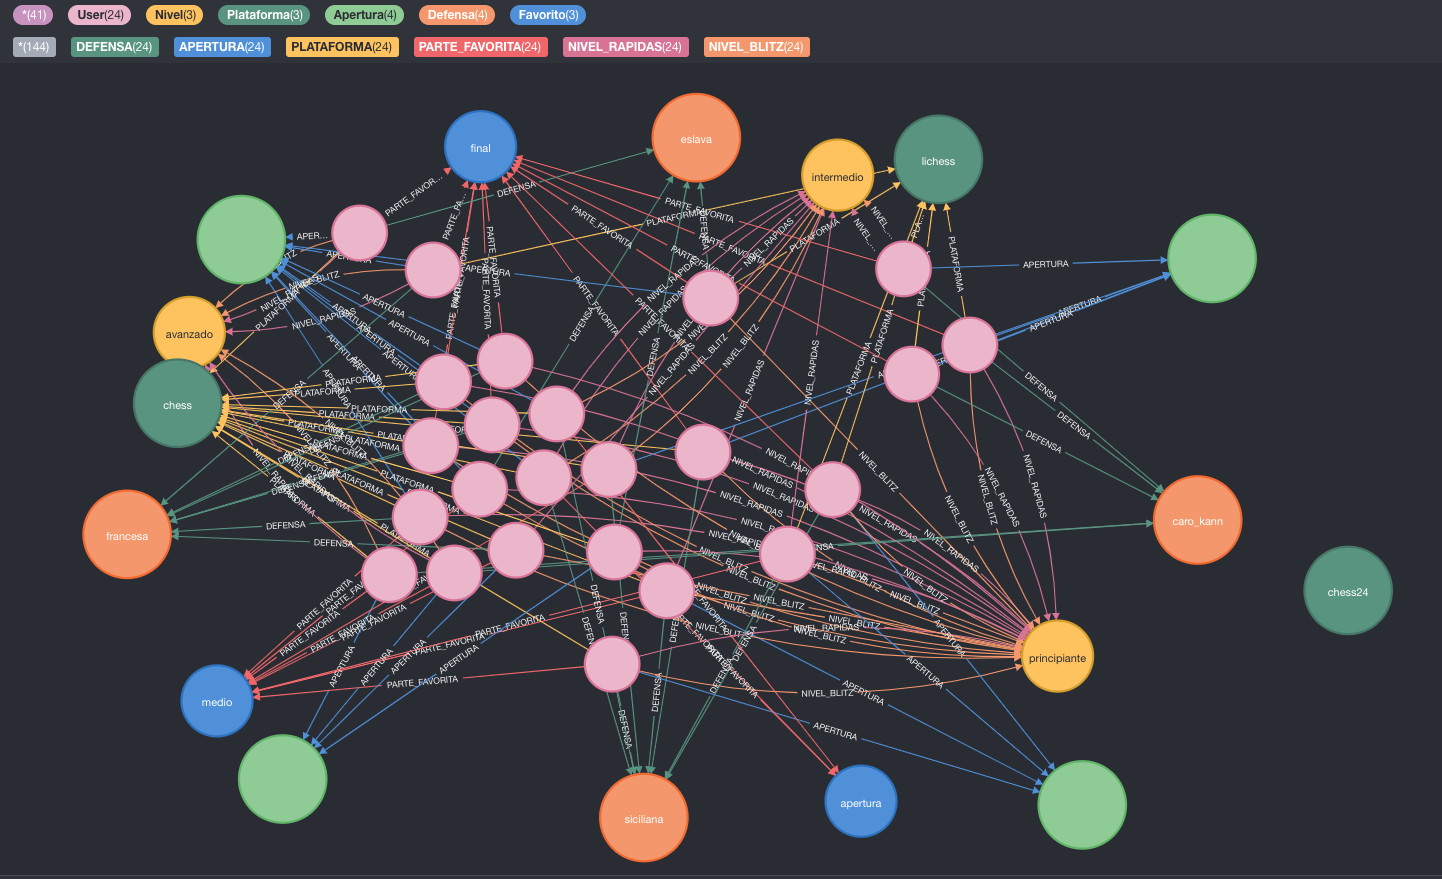
\includegraphics[scale=0.35]{/Users/rudiks/Git/Grafos/Documentación/Proyecto - Fase 2/Images/DB.png}
\end{center}

\section{¿Cómo el emplear el sistema de recomendaciones?}
\begin{tcolorbox}[colback=gray!15,colframe=black!1!black,title=ADVERTENCIA]
	El programa NO tiene programación defensiva, por lo que se requiere ser cuidadoso al ingresar los números solicitados. 
	\end{tcolorbox}

\begin{enumerate}
	\item Instalar \textit{Neo4J Desktop}. 
	\item Crear una base de datos. (Guardar la contraseña de la base de datos). 
	\item Abrir los archivos de Python. 
	\begin{enumerate}
		\item Dirigirse al archivo \begin{verbatim}: 
			main.py
		\end{verbatim}
	\item Posteriormente, en la primera línea de código modificar los siguiente: 
		\begin{lstlisting}
			DATABASE = DB.DB("PORT DE SU BASE DE DATOS", "neo4j", "CONTRASENA")	
			\end{lstlisting}
	\item Correr el programa. 
	\end{enumerate}
\item El sistema de recomendaciones es la primera opción que apecera en el menú mostrado. 
\begin{enumerate}
	\item Selecccionar en que modalidad quiere una recomendación.
	\item El programa le hará una recomendación de las aperturas/defensas basado en su nivel.
\end{enumerate}
\end{enumerate}

\section{Documentación de pruebas hechas con usuarios.}

Se les mostró la funcionalidad del programa a 5 miembros del Club de Ajedrez de la Universidad del Valle de Guatemala y posteriormente se les hizo una encuesta con las siguientes preguntas: 
\begin{enumerate}
	\item Luego de la corta explicación del programa, ¿qué tan complejo considera lo considera?
	\item ¿Considera que se cumplió el objetivo de crear un sistema de recomendaciones?
	\item ¿Las recomendaciones de aperturas le hacen sentido?
	\item ¿Las recomendaciones de defensas le hacen sentido?
	\item Si usted fuera un nuevo miembro del club, ¿considera que le sería de utilidad?
\end{enumerate}

* Considérese: (1) Deficiente y (5) Excelente. 

\subsection{Respuestas de los usuarios.}
\begin{table}[h]
	\centering
	\begin{tabular}{|c|c|c|c|c|c|}
		\hline
		PREGUNTA   & \textbf{1} & \textbf{2} & \textbf{3} & \textbf{4} & 5 \\ \hline
		\textbf{1} &            &            & 2 votos           & 3 votos         &   \\ \hline
		\textbf{2} &            &     1 voto       &  3 votos          &   1 voto         &   \\ \hline
		\textbf{3} &            &            &            &    2 votos        & 3 votos \\ \hline
		\textbf{4} &            &            & 1 voto        &  2 votos           &  2 votos \\ \hline
		\textbf{5} &            &            &   1 voto        &      4 votos     &   \\ \hline
	\end{tabular}
\end{table}



%---------------------------
%\bibliographystyle{apalike}
%\bibliography{sample.bib}

\end{document}